% 
% Lecture Template for ME3050 -  Dynamics Modeling and Controls - Tennessee Technological University
%
% Spring 2020 - Summer 2020
% Tristan Hill, May 07, 2020
% Module 3 - Newton's Approach 
% Topic 2 - The Velocity Model 
%

\documentclass{beamer}                         % for presentation (has nav buttons at bottom)
%\documentclass[handout]{beamer}  % for handout 
\usepackage{beamerthemesplit}
\usepackage{amsmath}
\usepackage{listings}
\usepackage{multicol}
\usepackage{framed}

\beamertemplateballitem

% custom colors
\definecolor{TTUpurple}{rgb}{0.3098, 0.1607, 0.5176} % TTU Purple (primary)
\definecolor{TTUgold}{rgb}{1.0000, 0.8666, 0.0000} % TTU Gold (primary) 
\definecolor{mygray}{rgb}{.6, .6, .6}
\definecolor{mypurple}{rgb}{0.6,0.1961,0.8}
\definecolor{mybrown}{rgb}{0.5451,0.2706,0.0745}
\definecolor{mygreen}{rgb}{0, .39, 0}
\definecolor{mypink}{rgb}{0.9960, 0, 0.9960}

% color commands
\newcommand{\R}{\color{red}}
\newcommand{\B}{\color{blue}}
\newcommand{\BR}{\color{mybrown}}
\newcommand{\K}{\color{black}}
\newcommand{\G}{\color{mygreen}}
\newcommand{\PR}{\color{mypurple}}
\newcommand{\PN}{\color{mypink}}

\setbeamercolor{palette primary}{bg=TTUpurple,fg=TTUgold}
\setbeamercolor{palette secondary}{bg=black,fg=TTUgold}
\setbeamercolor{palette tertiary}{bg=black,fg=TTUpurple}
\setbeamercolor{palette quaternary}{bg=TTUgold,fg=black}
\setbeamercolor{structure}{fg=TTUpurple} % itemize, enumerate, etc
\setbeamercolor{section in toc}{fg=TTUpurple} % TOC sections

%\usefonttheme{professionalfonts}

\newcommand{\LNUM}{3\hspace{2mm}} % Lecture Number 

\newcommand{\Lagr}{\mathcal{L}} % lagrangian

\newcommand{\vspccc}{\vspace{6mm}\\} % large vertical space
\newcommand{\vspcc}{\vspace{4mm}\\}   % medium vertical space
\newcommand{\vspc}{\vspace{2mm}\\}     % small vertical space

\newcommand{\hspcccc}{\hspace{10mm}} % large horizontal space
\newcommand{\hspccc}{\hspace{6mm}} % large horizontal space
\newcommand{\hspcc}{\hspace{4mm}}   % medium horizontal space
\newcommand{\hspc}{\hspace{2mm}}     % small horizontal space

\author{ME3050 - Dynamics Modeling and Controls} % original formatting from Mike Renfro, September 21, 2004

\newcommand{\MNUM}{3\hspace{2mm}} % Module number
\newcommand{\TNUM}{3\hspace{2mm}} % Topic number 
\newcommand{\moduletitle}{Newton's Approach }
\newcommand{\topictitle}{The Velocity Model } 

\newcommand{\sectiontitleI}{Example Problem - Quadcoptor Model}
\newcommand{\sectiontitleII}{Mathematical Modeling}
\newcommand{\sectiontitleIII}{Newton's Second Law Approach}
\newcommand{\sectiontitleIV}{Derived Equations of Motion}

\title{Module \MNUM - \moduletitle}

\date{Mechanical Engineering\vspc Tennessee Technological University} 

\begin{document}

\lstset{language=MATLAB,basicstyle=\ttfamily\small,showstringspaces=false}

\frame{\titlepage \center\begin{framed}\Large \textbf{Topic \TNUM - \topictitle}\end{framed} \vspace{5mm}}

% Section 0: Outline
\frame{

\large \textbf{Topic \TNUM - \topictitle} \vspace{3mm}\\

\begin{itemize}
	\item \sectiontitleI		\vspc % Section I
	\item \sectiontitleII 	\vspc % Section II
	\item \sectiontitleIII 	\vspc %Section III
	\item \sectiontitleIV 	\vspc %Section IV
\end{itemize}
}

% Section I:
\section{\sectiontitleI}

\frame{
\frametitle{\sectiontitleI}

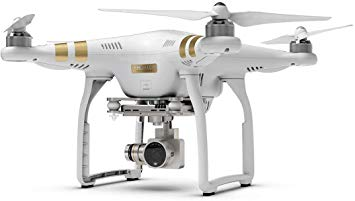
\includegraphics[scale=0.35]{dji_phantom.jpg}
\begin{framed}
\underline{Problem Statement} -  Derive the {\B equations of motion} using Newton's Second Law for the quadcopter velocity model.\vspc

\end{framed}

{\tiny Image: source needed}
}

% Section II:
\section{\sectiontitleII}

\frame{
\frametitle{\sectiontitleII}

First, consider the physical problem and list all simplifying assumptions necessary or desired. In general, the designed should start simple and add complexity incrementally. \vspc

\underline{Quadcopter Model Assumptions:}

\begin{enumerate}
\item
\item
\item
\end{enumerate}

}

% Section III:
\section{\sectiontitleIII}

\frame{
\frametitle{\sectiontitleIII}

\textbf{ \Large \underline{Newton's Second Law Approach} }\\
\begin{enumerate}
\item Draw a {\BR Free Body Diagram}\vspc
\item Make an {\G assumption of motion}\vspc
\item Determine all {\B forces} acting on the system and their {\B directions}. \vspc
\item Write {\PR Newton's second law} for the appropriate DOF. \vspc\
\item Re-write the ODE in the {\PN standard form} of a system equation.
\end{enumerate}

}

\frame{
\frametitle{\sectiontitleIII \hspace{1mm} - Steps 1,2 and 3}


}
	
\frame{
\frametitle{\sectiontitleIII \hspace{1mm} - Steps 4,5}


\begin{tabular}{ccc}
Translation:&$\Sigma {\bf F}=m{\bf a}$&$ \Sigma F_x=ma_x$\\
&&$\Sigma F_y=ma_y$\\
&&$\Sigma F_z=ma_z$ \\
&&\\
Rotation: &$\Sigma {\bf M}=I_o{\bf \alpha}$&$\Sigma M_o=I_o\alpha_z$\\
\end{tabular}

}	
	
% Section IV:
\section{\sectiontitleIV}

\frame{
\frametitle{\sectiontitleIV}



}	
	
\end{document}





